\chapter{Reconstruction of the top-pair Kinematics}\label{chapt:kinReco}

The two neutrinos are not detected, thus additional information and
assumptions are needed to determine the full final state kinematics of the $t\bar{t}$ system reconstructed in the dilepton decay channel.
This section describes the method used for the full reconstruction. The analytical solution of the
kinematic equations (sec. \ref{sec:MatBg}) as well as a performance test of the method 
(sec. \ref{sec:SolSer} -- \ref{sec:kinRecPerf}) are discussed.

\section{Analytical Solution of Kinematic Equations}\label{sec:MatBg}

The presence of two undetected neutrinos introduces six unknowns  (three momentum components of each neutrino)
for the $t\bar{t}$ system in the dilepton final state.
The following constraints are being used:

\begin{itemize}
 \item \textit{t and $\bar{t}$ masses} ($m_{t}$ and $m_ {\bar{t}}$) are assumed to be equal and constrained to the same value of 172.5 GeV\cite{PDG-2012};
 \item The whole missing transverse energy $E_{T}^{miss}$ of the event is assumed to arise entirely
 from the two neutrinos from the $t\bar{t}$ decay;
 \item \textit{The $W^{\pm}$ masses} ($m_{W\pm}$) are assumed to be known. As $W^{\pm}$ are resonances with a very small lifetime, their masses 
 are distributed according to a Breit-Wigner function. For this reconstruction, the $W^{\pm}$ masses are set to values randomly taken 
 from the generator Breit-Wigner $W^{\pm}$ mass spectrum.
\end{itemize}

These assumptions lead to a system of six equations which describe the conservation of energies and momenta:

\begin{align}\label{alg:LS1}
 E^{miss}_{T_{x}} & =  p_{\nu_{x}} + p_{\bar{\nu}_{x}} \\
 %
 E^{miss}_{T_{y}} & =  p_{\nu_{y}} + p_{\bar{\nu}_{y}} \\
 %
 m^{2}_{W^{+}} & = (E_{l^{+}} + E_{\nu})^{2} - (p_{l^{+}_{x}} + p_{\nu_{x}})^{2} - (p_{l^{+}_{y}} + p_{\nu_{y}})^{2} - (p_{l^{+}_{z}} + p_{\nu_{z}})^2 \\
 %
 m^{2}_{W^{-}} & = (E_{l^{-}} + E_{\bar{\nu}})^{2} - (p_{l^{-}_{x}} + p_{\bar{\nu}_{x}})^{2} - (p_{l^{-}_{y}} + p_{\bar{\nu}_{y}})^{2} - (p_{l^{-}_{z}} + p_{\bar{\nu}_{z}})^2 \\
 % 
 m_{t}^{2} & = (E_{b} + E_{l^{+}} + E_{\nu})^{2} - (p_{b_{x}} + p_{l^{+}_{x}} + p_{\nu_{x}})^2 \nonumber \\
           & - (p_{b_{y}} + p_{l^{+}_{y}} + p_{\nu_{y}})^2 - (p_{b_{z}} + p_{l^{+}_{z}} + p_{\nu_{z}})^2 \\
 %
 m_{\bar{t}}^{2} & = (E_{\bar{b}} + E_{l^{-}} + E_{\bar{\nu}})^{2} - (p_{\bar{b}_{x}} + p_{l^{-}_{x}} + p_{\bar{\nu}_{x}})^2 \nonumber \\
                 & - (p_{\bar{b}_{y}} + p_{l^{-}_{y}} + p_{\bar{\nu}_{y}})^2 - (p_{\bar{b}_{z}} + p_{l^{-}_{z}} + p_{\bar{\nu}_{z}})^2\label{alg:LS6} 
\end{align}

Here the $E_{l^{\pm}}$ and $p_{l^{\pm}_{x,y,z}}$ correspond to the lepton(antilepton) energy and momentum components respectively; 
$E_{b/\bar{b}}$ and $p_{b/\bar{b}_{x,y,z}}$ are the $b$/$\bar{b}$-jet energy and momentum components respectively; the $E^{miss}_{T_{x,y}}$ are
the two components of the missing transverse energy; the $p_{\nu/\bar{\nu}_{x,y,z}}$ are the neutrino (antineutrino) momenta components.
The neutrino energies $ E_{\nu/\bar{\nu}}$ are determined from their momenta:

\begin{equation}
 E_{\nu/\bar{\nu}}^{2} = p_{\nu/\bar{\nu}_{x}}^{2} + p_{\nu/\bar{\nu}_{y}}^{2} + p_{\nu/\bar{\nu}_{z}}^{2}
\end{equation}

The quantities $E_{l^{\pm}}$, $p_{l^{\pm}_{x,y,z}}$, $E_{b/\bar{b}}$, $p_{b/\bar{b}_{x,y,z}}$ and $E^{miss}_{T_{x,y}}$ are reconstructed from the detector (as described in chapter \ref{chapt:event_selection})
and $p_{\nu/\bar{\nu}_{x,y,z}}$ are the unknowns.

An analytical solution of the system of equations (\ref{alg:LS1}--\ref{alg:LS6}) was proposed in \cite{LSpaper}. After a number of transformations
the system is reduced to a fourth order polynomial equation for the neutrino momentum component $p_{\nu_{x}}$:

\begin{equation}\label{eq:eqLSf}
 0 = h_{0} p_{\nu_{x}}^{4} + h_{1} p_{\nu_{x}}^{3} + h_{2} p_{\nu_{x}}^{2} + h_{3} p_{\nu_{x}} + h_{4},
\end{equation}

where the coefficients $h_{0} - h_{4}$ \cite{LSpaper, LSerrat} depend on the missing transverse energy $E_{T}^{miss}$ and four-momenta of the
leptons, antileptons, $b$- and $\bar{b}$-jets. 

There can be up to four solutions for equation \ref{eq:eqLSf}. This equation (in case if the coefficients $h$ are such that the equation can't be simplified to the third, second
or first order) can not have analytically three or one real solutions as proven in \cite{LSpaper}, thus, it is expected to get either two or four solutions. However, due to the 
limited computing accuracy, there may be cases when two solutions are indistinguishable and treated as one. This phenomenon can create three out of four or one out of two solutions.

The distribution of the number of solutions for the generated \MG + \PYTHIA $t\bar{t}$ signal sample 
is shown in Fig. \ref{fig:LSNsol}. Two (four) solutions per event are expected in approx. 80$\%$ (20\%) of the cases.
The cases, when there are one or three solutions found, have a rate of about 0.1\%.

\begin{figure}[t]
  \centering
  \includegraphics[width=0.8\textwidth]{/home/dolinska/Dropbox/desy_plots/Thesis/Jenya/05_kinReco/plots/Nsolutions.pdf}
  \caption{Number of solutions of the equation \ref{eq:eqLSf}. The distribution is normalized to unity. The information used for this plot is taken
  from the generated \MG + \PYTHIA $t\bar{t}$ signal for this analysis.}
  \label{fig:LSNsol}
\end{figure}


% Under the real conditions a sizable amount of the events will find no solutions of the kinematic equations (\ref{alg:LS1}--\ref{alg:LS6})
% because of an imperfect reconstruction of the detector objects. But in the other cases there is a possibility to find up to four solutions.

\section{Ambiguity and Detector Effects Treatment}\label{sec:SolSer}

There are several problems arising during the $t\bar{t}$ dilepton final state kinematics reconstruction:

\begin{itemize}
 \item \textit{Fluctuations of measurement}. There might be no real solutions of the equation \ref{eq:eqLSf} found for a combination
 of leptons, jets and missing transverse energy arising from the $t\bar{t}$ system due to reconstruction effects, e.g. detector resolution,
 jet overlapping, badly reconstructed missing transverse energy, etc. Due to these effects, the kinematics of the reconstructed 
 jets and leptons may be estimated with distortions. Thus, the input parameters of the equations \ref{eq:eqLSf} will be distorted,
 which will result in the impossibility to find a real (physical) solution of the equations.
 %
 \item \textit{Multiple solutions of the kinematic equations}. As discussed in section \ref{sec:MatBg} the equation \ref{eq:eqLSf}
 has up to four mathematical solutions while only one of them corresponds to the correct kinematics of the neutrino.
 %
 \item \textit{Multiple combinations of leptons and jets}. An event with a $t\bar{t}$ decaying to a dilepton final state has at least two leptons and two
 $b$-jets. However there is a priori no information if a $b$-jet originates from the $t$ or the $\bar{t}$. For this reason each $b$-jet candidate is being 
 paired to one of the leptons, and then to another
 to form a $t$ or $\bar{t}$ candidate. Thus an event with two leptons and two $b$-jets has two possible $t\bar{t}$ candidates. In case of further jets
 in the event, the number of $t\bar{t}$ candidates can be up to $N_{jet}!$, where $N_{jet}$ is the jet multiplicity.
\end{itemize}

% The last two challenges have different nature but boths cause the same issue of multiple possible $t\bar{t}$ candidates, thus they can be treated together.

\subsection{Fluctuations of measurements}\label{ssec:smear}

The problem of rescuing the events which are lost due to fluctuations is solved by varying the measured objects energies and
momentum directions. This increases the efficiency of finding a solution of the system of equations (\ref{alg:LS1}--\ref{alg:LS6}) (see Appendix \ref{appendix:smear}). 
The idea was implemented by reconstructing each event 100 times, each time varying relevant observables according to their resolution determined from the Monte Carlo simulation.
The energies and directions of leptons and jets are smeared. All variations are done randomly, independently and simultaneously for each quantity.

The energy variation was performed through multiplication of the reconstructed energy value
by a correction factor determined from the detector energy response distribution $f = \frac{E_{true}}{E_{reco}}$. Here $E_{reco}$ is the reconstructed lepton 
or $b$-jet energy taken from the MC signal simulation and $E_{true}$ is the true energy of the same object on the particle level. The response distributions 
which are used for the random choice of the correction factors are shown in Fig. \ref{fig:fE}. The response is determined from 
the signal MC simulation using $b$-jets and leptons matched to the particle level $b$-quarks and leptons arising from the decay chain 
$t \rightarrow WB \rightarrow l\nu b$. The binning of the response distribution was chosen such that the bin width would be smaller than the 
root mean square (RMS) deviation of these distributions. The distributions shown in Fig. \ref{fig:fE} have the bin width three times
smaller than the RMS\footnote{For this estimation the RMS was determined for the range $[0.5\;..\;1.5]$ for the response distribution
of jets and $[0.9\;..\;1.2]$ for the response distribution of leptons.}.

The response distributions for electrons and muons separately almost do not differ. Their shape is similar, the mean value is the same and 
the RMS deviation determined in the region $[0.9\;..\;1.2]$ is about $5\%$ different. That is why for simplicity the combined distribution
for electrons and muons (shown in Fig. \ref{fig:fE}) was used for this analysis.

If, due to the energy smearing, the lepton or jet $p_{T}$ is reduced to the value beyond the selection criteria (see sec. \ref{sec:sel}), they are still accepted.

\begin{figure}[h]
\centering
\begin{subfigure}
  \centering
  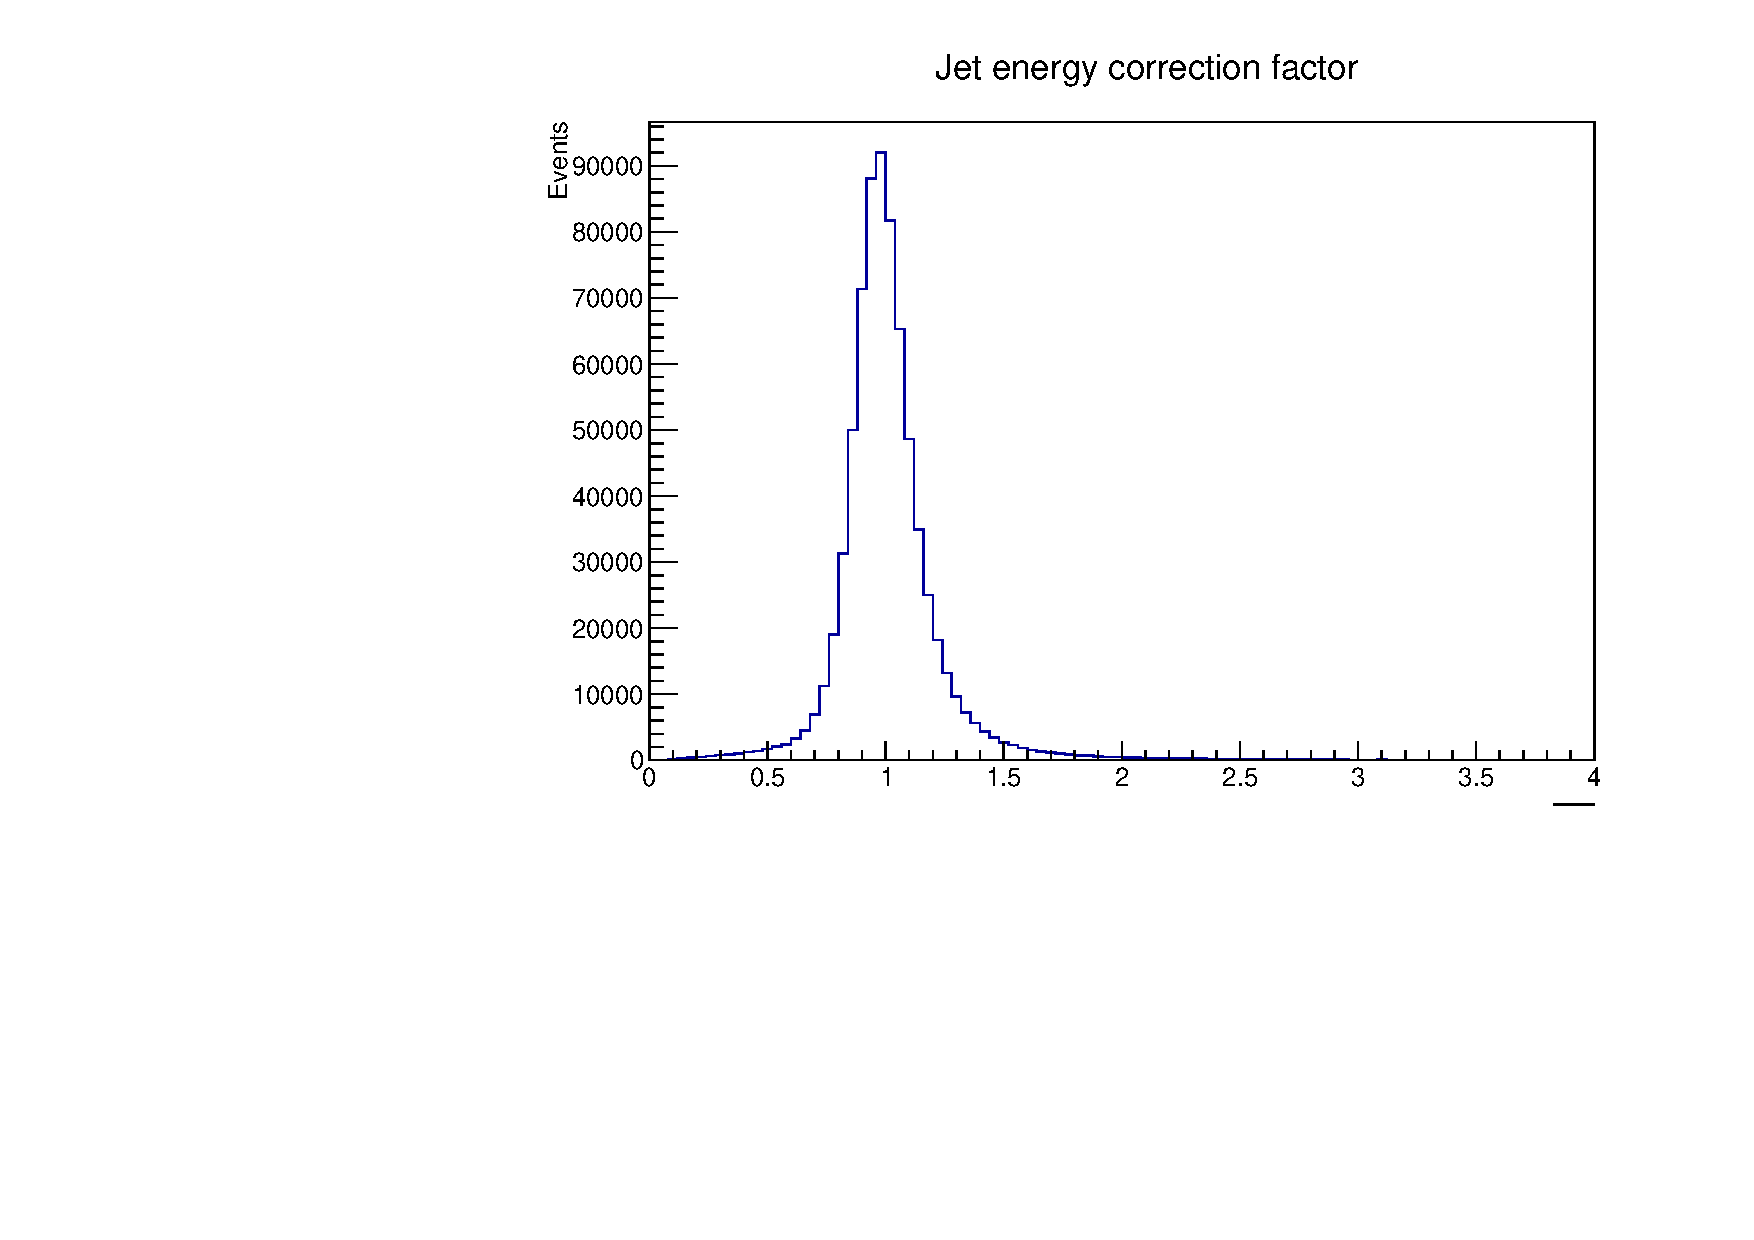
\includegraphics[width=0.48\textwidth]{/home/dolinska/Dropbox/desy_plots/Thesis/Jenya/05_kinReco/plots/fE_jet.pdf}
\end{subfigure}
\begin{subfigure}
  \centering
  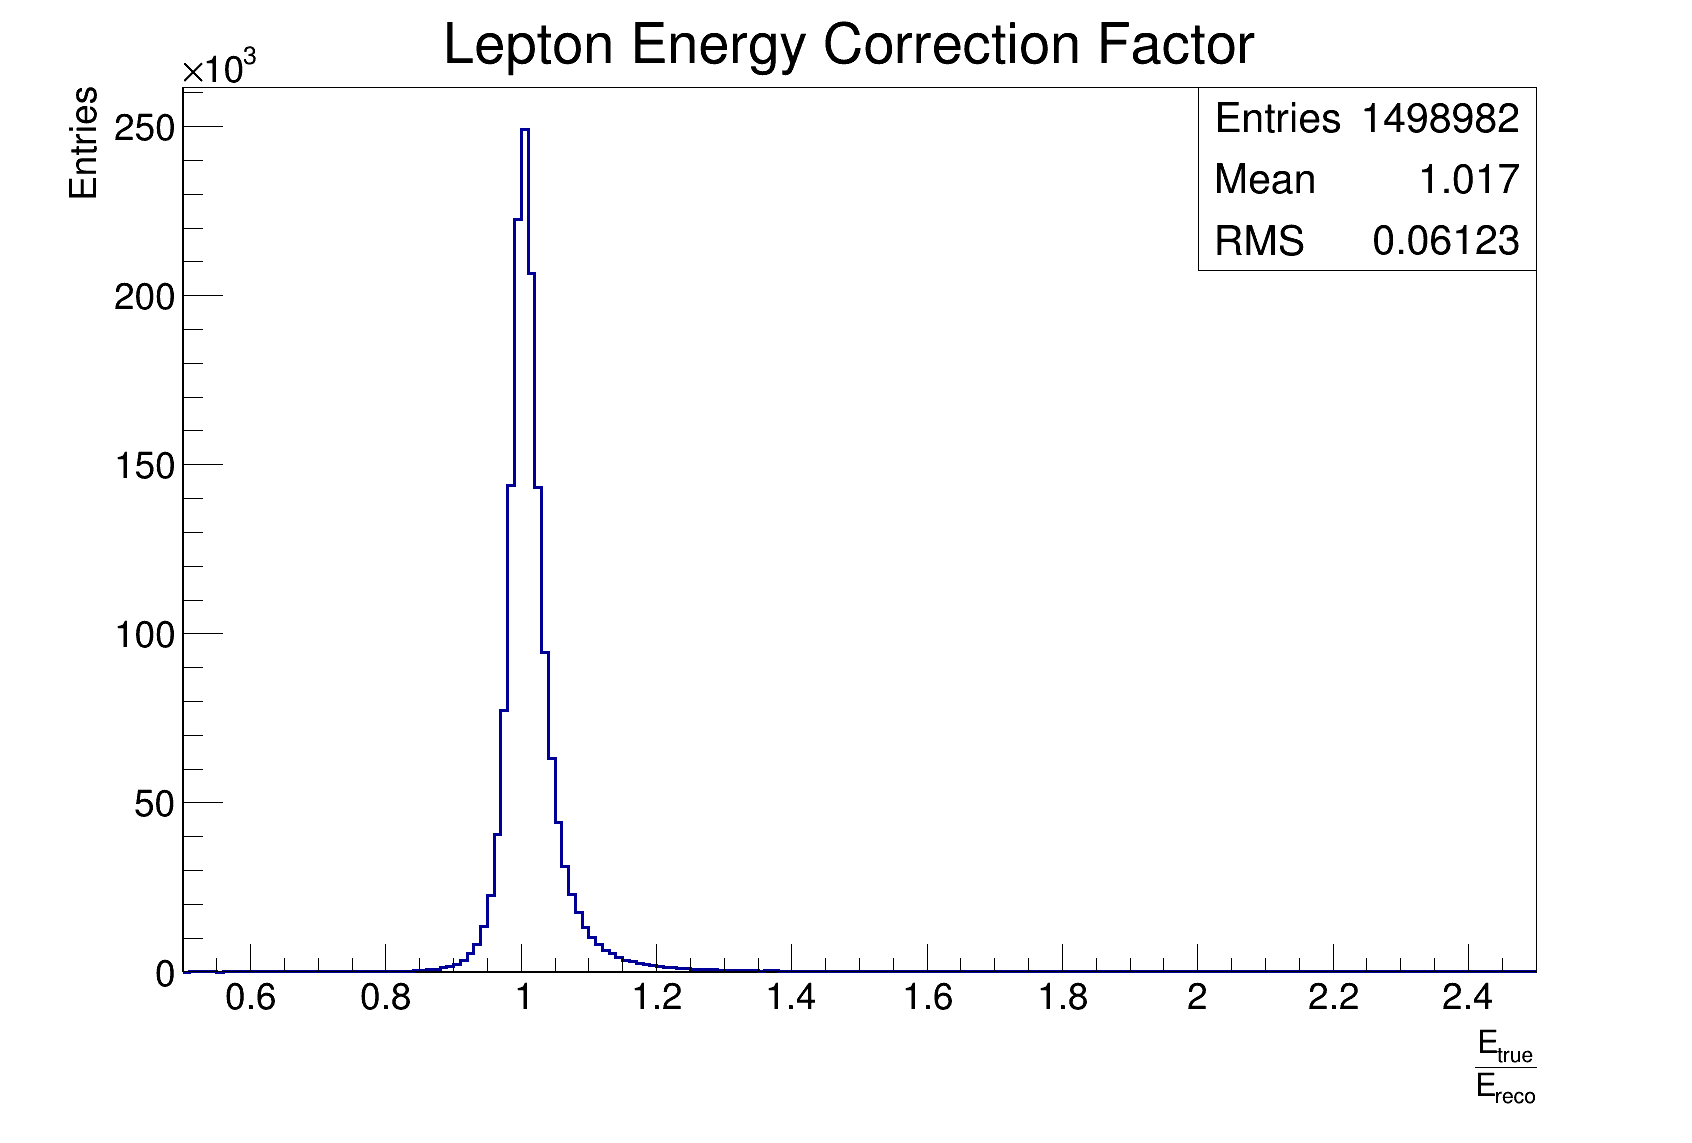
\includegraphics[width=0.48\textwidth]{/home/dolinska/Dropbox/desy_plots/Thesis/Jenya/05_kinReco/plots/fE_lep.pdf}
\end{subfigure}
\begin{subfigure}
  \centering
  \includegraphics[width=0.48\textwidth]{/home/dolinska/Dropbox/desy_plots/Thesis/Jenya/05_kinReco/plots/fE_jet-log.pdf}
\end{subfigure}
\begin{subfigure}
  \centering
  \includegraphics[width=0.48\textwidth]{/home/dolinska/Dropbox/desy_plots/Thesis/Jenya/05_kinReco/plots/fE_lep-log.pdf}
\end{subfigure}
\caption{Energy response distributions for $b$-jets (left) and for leptons (right) for the energy smearing in the kinematic
reconstruction of the top-quark kinematics. The plots are shown in linear scale (top) and logarithmic scale (bottom).}
\label{fig:fE}
\end{figure}

The directional smearing is applied by rotating the actual momentum vectors relatively to the nominal vector direction
as shown in Fig. \ref{fig:angleRot}. 
\begin{figure}[H]
 \centering
 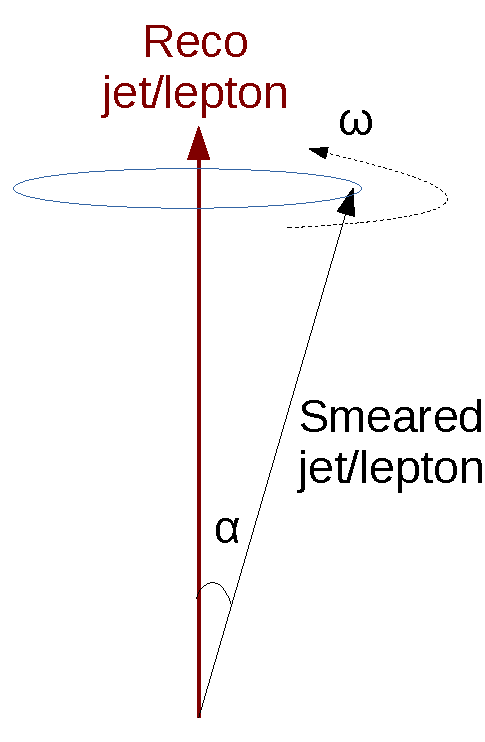
\includegraphics[width=0.2\textwidth]{05_kinReco/plots/angle_rot.pdf}
 \caption{Sketch of the directional smearing of leptons and jets as applied in the $t\bar{t}$ kinematic reconstruction.}
 \label{fig:angleRot}
\end{figure}

A smearing of the polar angle $\alpha$ is performed by choosing a random value from
the MC distributions presented in Fig. \ref{fig:dAngle}. The azimuthal angle $\omega$ is taken randomly from 0 to $2\pi$.
These distributions do not depend on the $\phi$ coordinate of leptons and $b$-quarks and have a slight dependence on $\eta$. For
example, for $b$-quarks with $\eta\;\in\;[-2.5\;..\;-1.5]$ the mean value of the distributions is 0.025 and RMS is 0.042,
while for the $b$-quarks with $\eta\;\in\;[-0.5\;..\;0]$ the mean value is 0.05 and RMS is 0.07.

\begin{figure}[t]
\centering
\begin{subfigure}
  \centering
  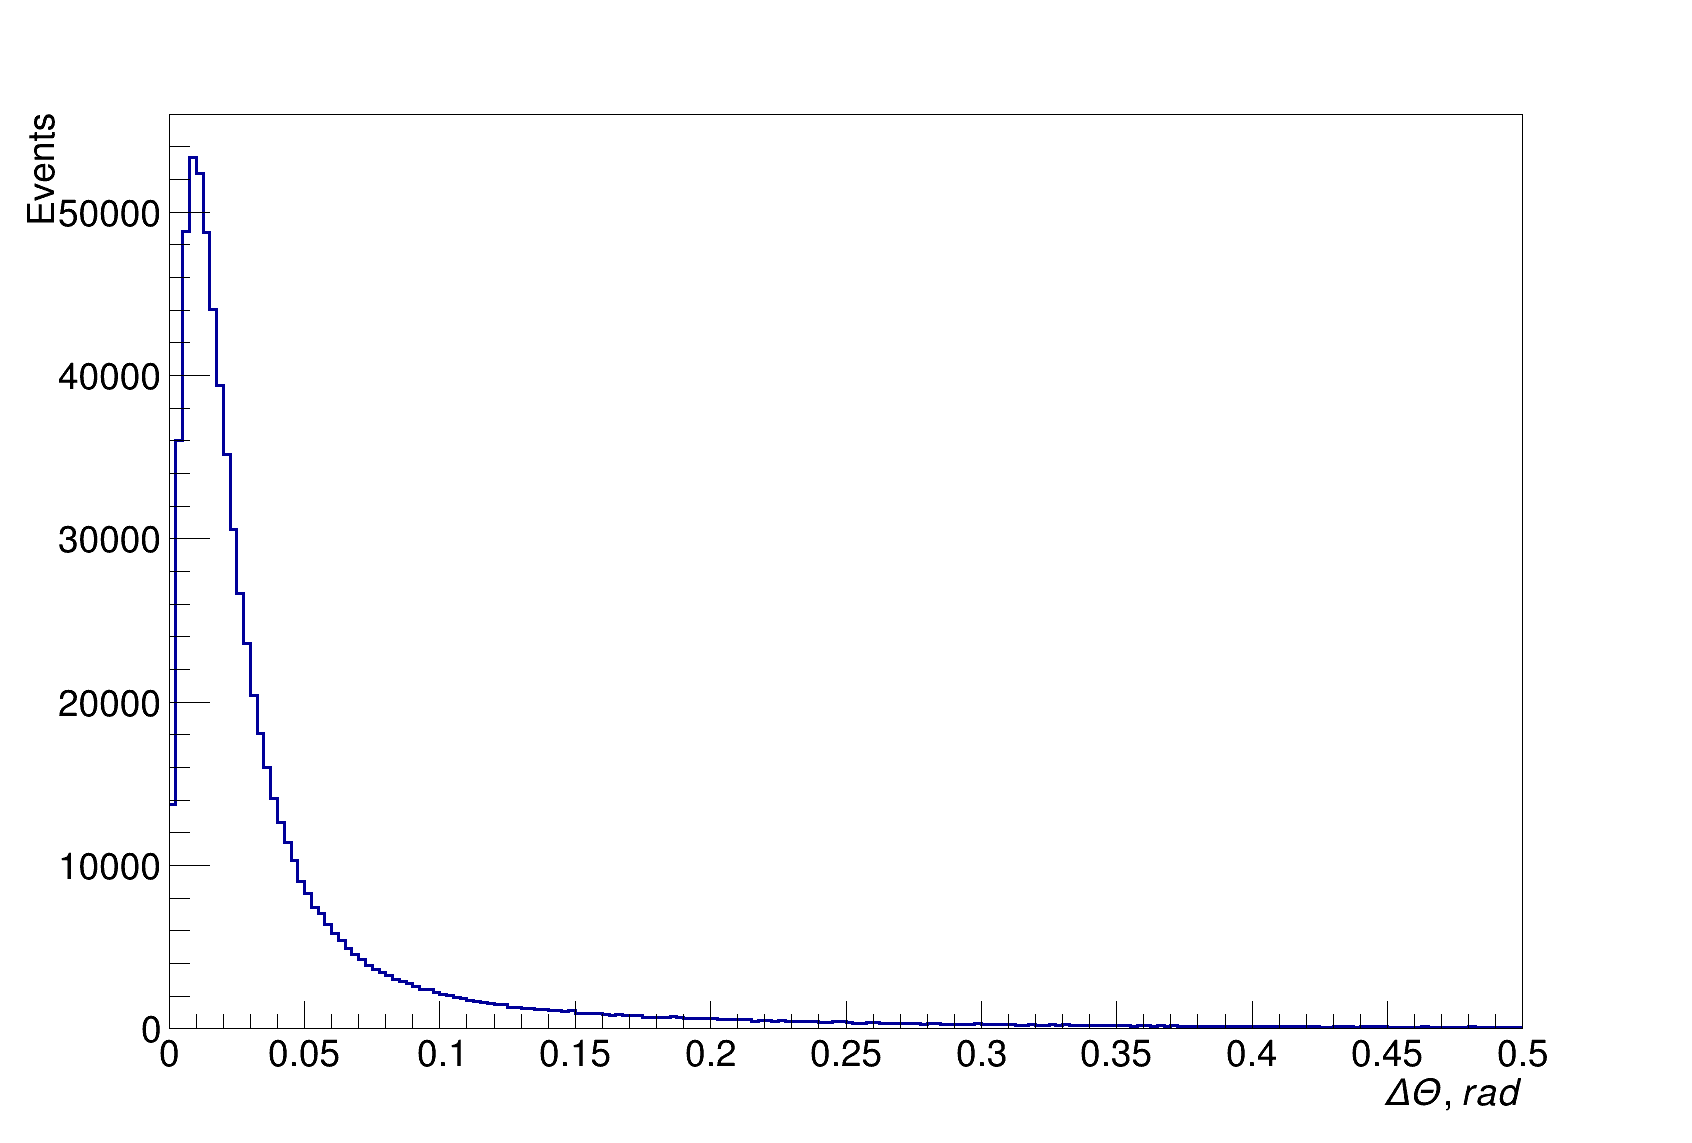
\includegraphics[width=0.48\textwidth]{/home/dolinska/Dropbox/desy_plots/Thesis/Jenya/05_kinReco/plots/dan_jet.pdf}
\end{subfigure}
\begin{subfigure}
  \centering
  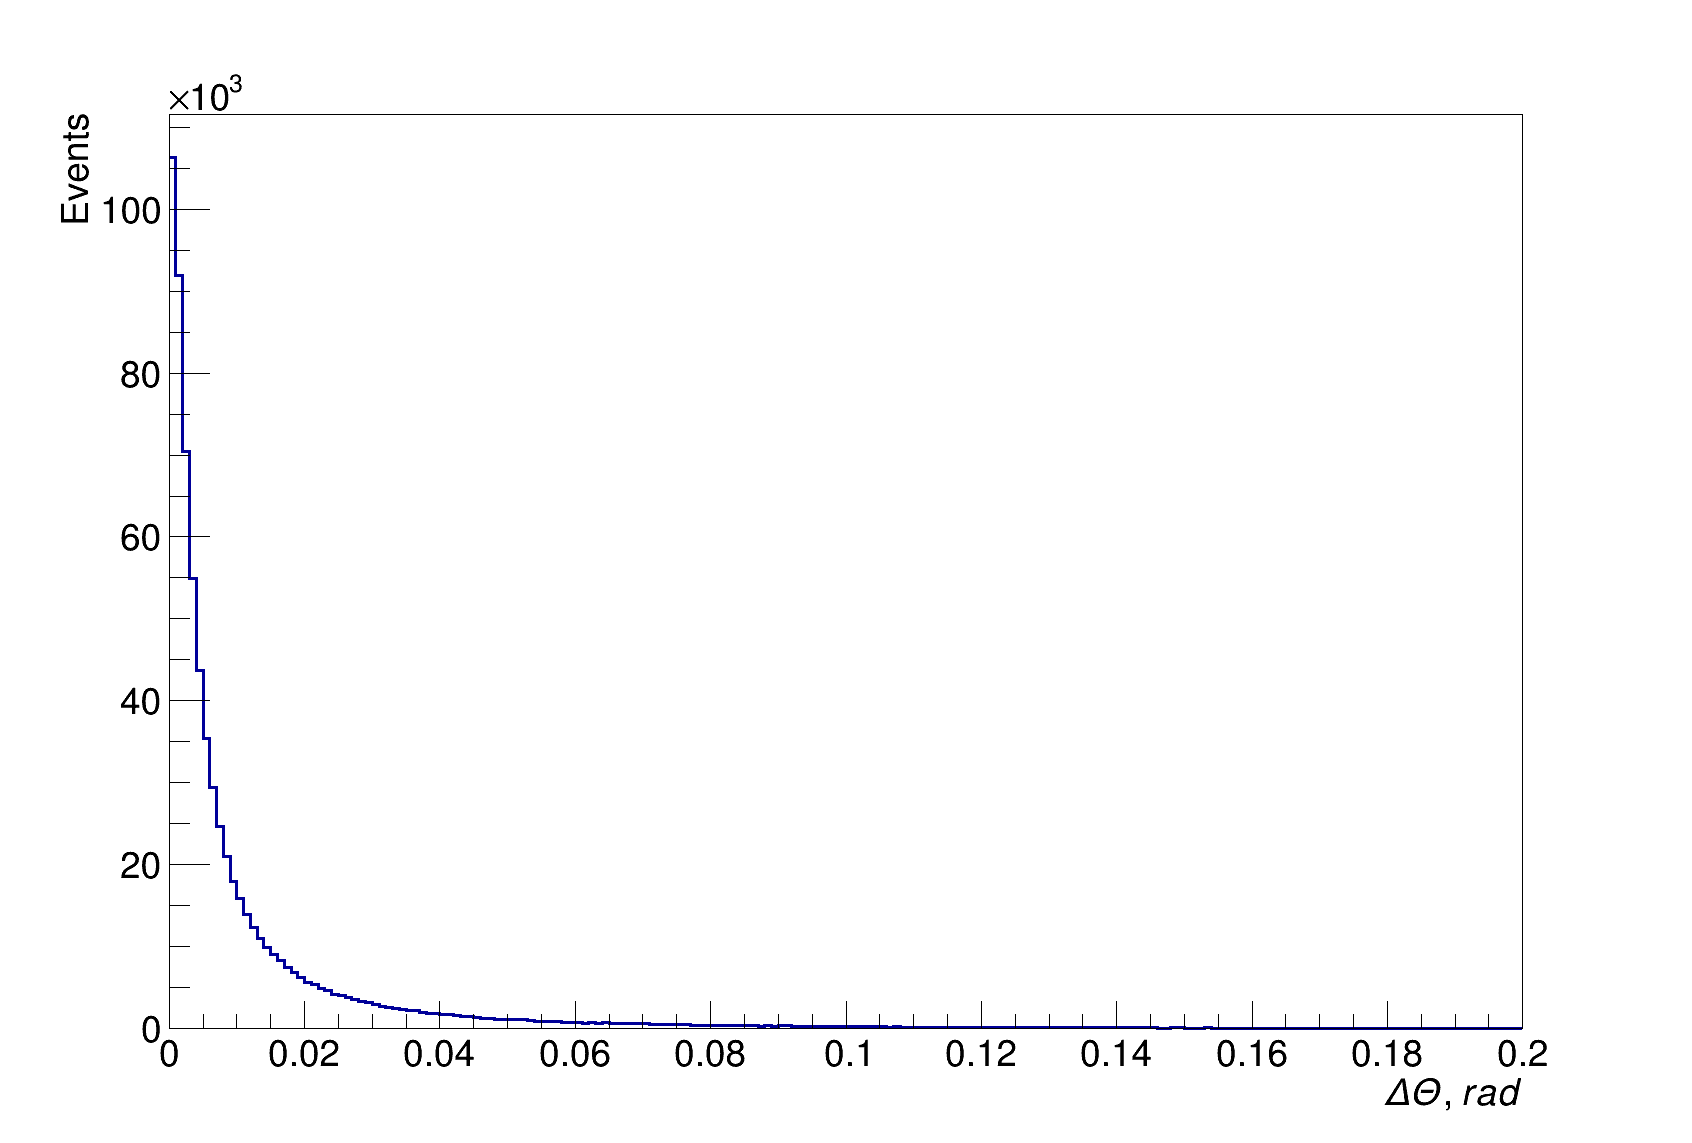
\includegraphics[width=0.48\textwidth]{/home/dolinska/Dropbox/desy_plots/Thesis/Jenya/05_kinReco/plots/dan_lep.pdf}
\end{subfigure}
\begin{subfigure}
  \centering
  \includegraphics[width=0.48\textwidth]{/home/dolinska/Dropbox/desy_plots/Thesis/Jenya/05_kinReco/plots/dan_jet-log.pdf}
\end{subfigure}
\begin{subfigure}
  \centering
  \includegraphics[width=0.48\textwidth]{/home/dolinska/Dropbox/desy_plots/Thesis/Jenya/05_kinReco/plots/dan_lep-log.pdf}
\end{subfigure}
\caption{Distributions of the angle between the particle level direction and the detector level direction.
The angle distribution for the $b$-quarks is shown on the left and for the leptons (electrons and muons) on the right.
The plots are shown in linear scale (top) and logarithmic scale (bottom).}
\label{fig:dAngle}
\end{figure}

In each of the 100 variations of the jet and lepton kinematics, the transverse missing energy $E_{T}^{miss}$ has to be recalculated. This is done
assuming the transverse energy component, which does not refer to the leptons and jets forming a $t\bar{t}$ candidate, to be constant. Thus the
missing transverse energy for the $i^{th}$ smearing will be expressed as following:

\begin{equation}\label{eq:weigh_av}
 E^{miss\;i}_{T_{x,y}} = E^{miss \; from \, reco}_{T_{x,y}} + p^{jets \; reco}_{x,y} + p^{leptons\;reco}_{x,y} - (p^{jets\;i}_{x,y} + p^{leptons\;i}_{x,y}).
\end{equation}

Here the $E^{miss \; from \, reco}_{T_{x,y}}$, $p^{jets \; reco}_{x,y}$ and $p^{leptons\;reco}_{x,y}$ are the missing transverse energy and momenta
components taken directly from the detector reconstruction (see chapt. \ref{chapt:event_selection} and \ref{chapt:event_sel}) without applying any 
variations; the $p^{jets\;i}_{x,y}$ and $p^{leptons\;i}_{x,y}$ are the smeared jets and leptons momenta respectively on the $i^{th}$ of the 100 
variation step.

\subsection{Single solution choice}

The equation \ref{eq:eqLSf} is solved for every of the 100 event reconstructions. Each equation may have up to four solutions, thus each event
has up to ($100 \times 4 \times N_{jet}!$) reconstructed $t\bar{t}$ candidates (the factor $N_{jet}!$ has already been discussed is sec. \ref{sec:SolSer}). 
To obtain one $t\bar{t}$ pair out of this candidate variety, the following steps are applied:

\begin{itemize}

 \item [--] First, the single combination of leptons and jets is selected (getting rid of the combinatorics part $N_{jet}!$). If solution with 
 two $b$-tagged jets (see sec. \ref{ssec:bTag}) are found then combinations with only one $b$-tagged jet are not considered. Then for each 
 combination a following weight is assigned:
 
 \begin{equation}\label{eq:mblw}
  \omega = \sum_{i=1}^{100} \omega^{i} = \sum_{i=1}^{100} \omega^{i}_{m^{\bar{l}b}} \cdot \omega^{i}_{m^{l\bar{b}}}.
 \end{equation}

 Here $i$ is the number of smearing of the event (see sec. \ref{ssec:smear}), $m^{\bar{l}b}$ and $m^{l\bar{b}}$ are the reconstructed 
 invariant masses of the smeared lepton-jet pairs from the top and the anti-top decays, respectively. These weights are calculated 
 according to spectrum of the correct lepton-jet pairs in top decays obtained from the signal MC on the particle level after all kinematic 
 cuts described in chapter \ref{chapt:event_sel}. The spectrum is shown in Fig. \ref{fig:mlb}. A combination of leptons and jets with 
 the highest weight $\omega$ is taken for the further analysis. This reduces the number of the possible candidates to maximum $100 \times 4$.
 
 \begin{figure}[t]
  \centering
  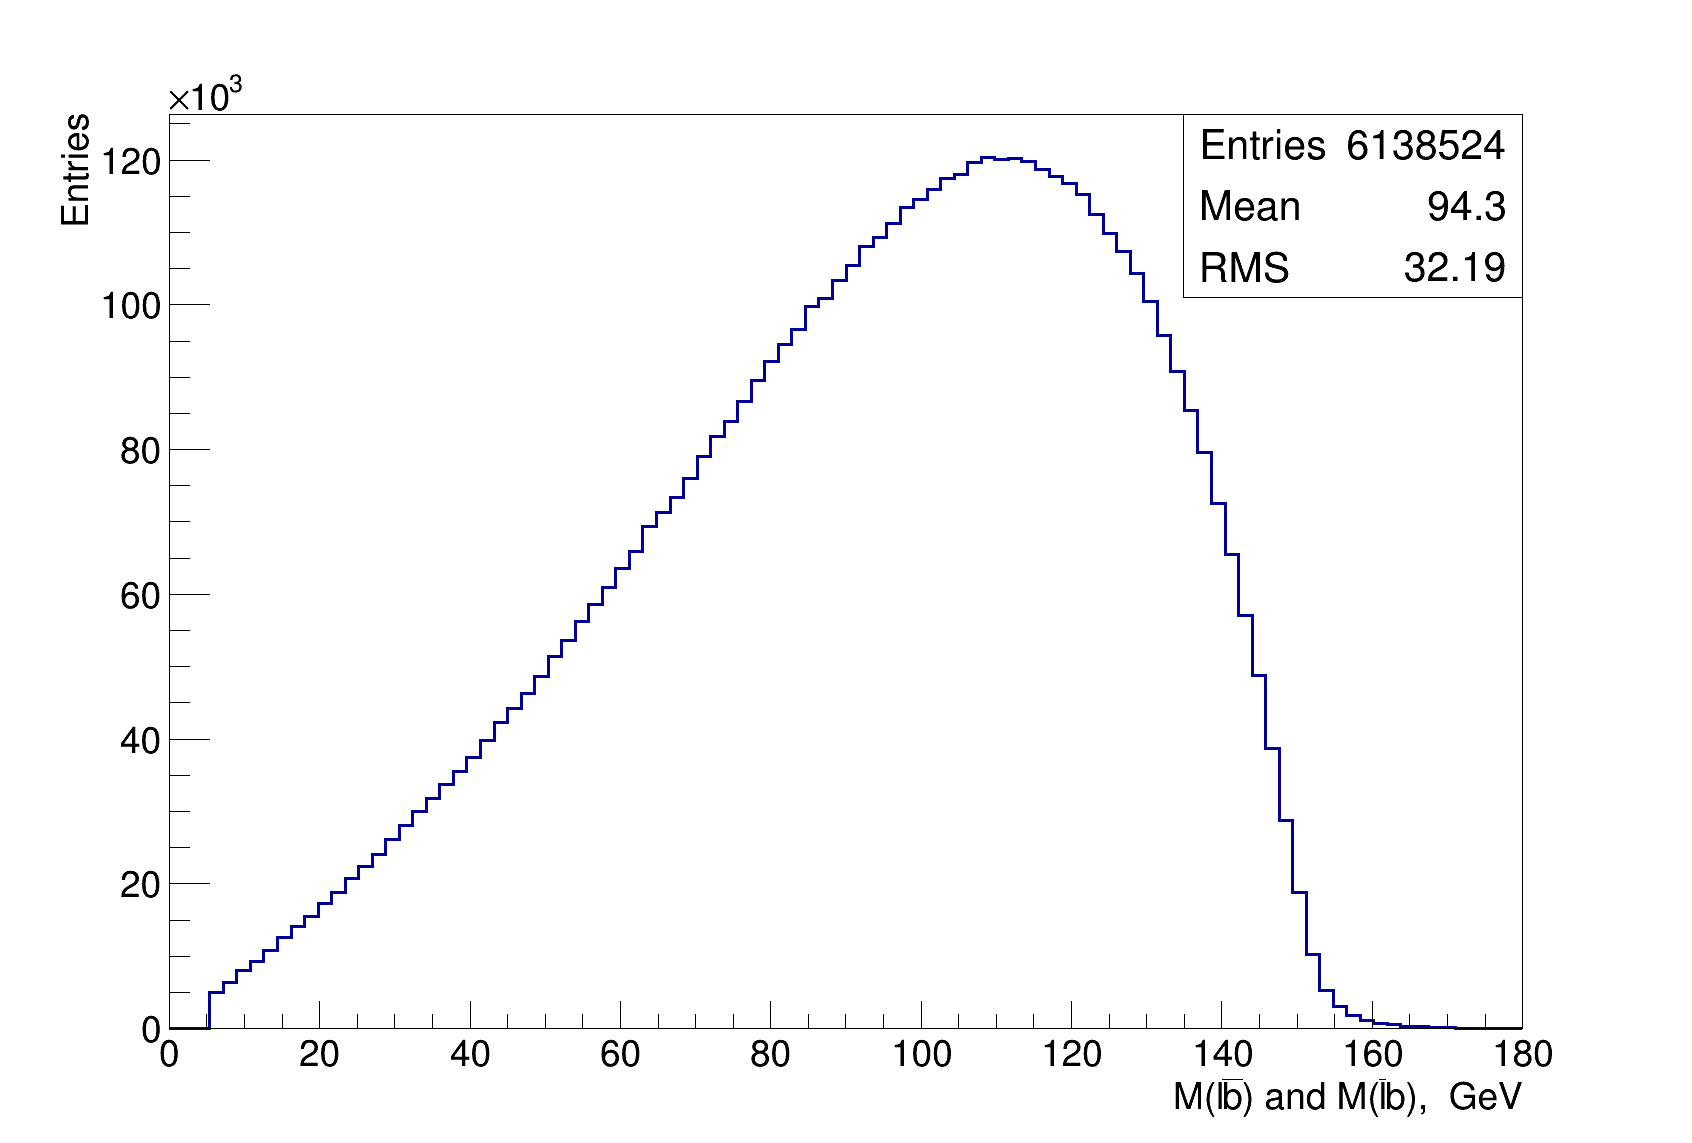
\includegraphics[width=0.8\textwidth]{05_kinReco/plots/mlb_distr.png}
  \caption{Distribution of the invariant mass of the lepton -- $b$-jet system originating from one $t/\bar{t}$-quark. This distribution is obtained from the
  generator level $t\bar{t}$ signal MC.}
  \label{fig:mlb}
 \end{figure}
 
 \item [--] For each of the four solutions of equation \ref{eq:eqLSf} the invariant mass of the $t\bar{t}$ pair, $m(t\bar{t})$, is calculated. Only
 the solution with the smallest $m(t\bar{t})$ is taken. The detailed study of the smallest $m(t\bar{t})$ criterion is presented in Appendix \ref{appendix:mtt}. 
%  This criterion was prior introduced in \cite{PhysRevD.73.112006}, where it was shown to
%  deliver for the correct lepton-jet assignment in most cases the correct solution.
 %
 \item [--] For the remaining up to 100 candidates (these number is related only to the energy and directional smearing, see sec. \ref{ssec:smear}), the $t$($\bar{t}$) 
 momentum is constructed as a weighted average of all smeared solutions as following:
 \begin{equation}
  \langle{\vec{p}(t/\bar{t})}\rangle = \frac{\sum\limits_{i=1}^{100} \omega_{i} \vec{p}(t/\bar{t})_i}{\omega}.
 \end{equation}
 Here $\vec{p}(t/ \bar{t})_{i}$ is the $t$ or $\bar{t}$ momentum three vector for the $i^{th}$ variation in the event. The weights ($\omega$ and $\omega_{i}$ are taken according 
 to the eq. \ref{eq:mblw}).
 In case that for the $i^{th}$ variation no solution of the kinematic equations is found, both weight and momentum three vector are set to zero. To complete the kinematics,
 the $t$ and $\bar{t}$ energies are calculated taking $\langle{\vec{p}(t/\bar{t})}\rangle$ and assuming the top mass $m(t) = m(\bar{t}) = $ 172.5 GeV.
\end{itemize}

\section{Performance}\label{sec:kinRecPerf}

Only the events in which solutions of kinematic equations are found are accepted for this analysis. 
In Fig. \ref{fig:EffSF} the efficiencies and scale factors (as defined in chapter \ref{chapt:event_sel}) for the $t\bar{t}$ kinematic reconstruction procedure 
depending on jet multiplicity in the event, lepton and $b$-jets kinematics and missing transverse energy for the data after the full event selection
(see sec. \ref{sec:sel}) and the $t\bar{t}$ signal simulation are shown. The integrated efficiency of the kinematic reconstruction method is 93 $\%$. One of
the identified sources (from the $t\bar{t}$ signal MC) is the effect that at least one $b$-jet from $t$ or $\bar{t}$ decay has failed the transverse
momentum or rapidity cut and instead a wrong jet was selected.
% The remaining 7\% inefficiency possibly originates from the events, where the kinematic reconstruction failed due to the 
% wrong jet choice or due to the detector resolution.

Overall, the scale factors 
show a flat behavior depending on different variables, thus a value of 0.99 for the scale factor is used for the analysis. This value was determined 
from the total number of reconstructed events in data and MC on reconstructed level ($t\bar{t}$ signal and all the background samples) before and
after kinematic reconstruction.

\begin{figure}[t]
\centering
\begin{subfigure}
  \centering
  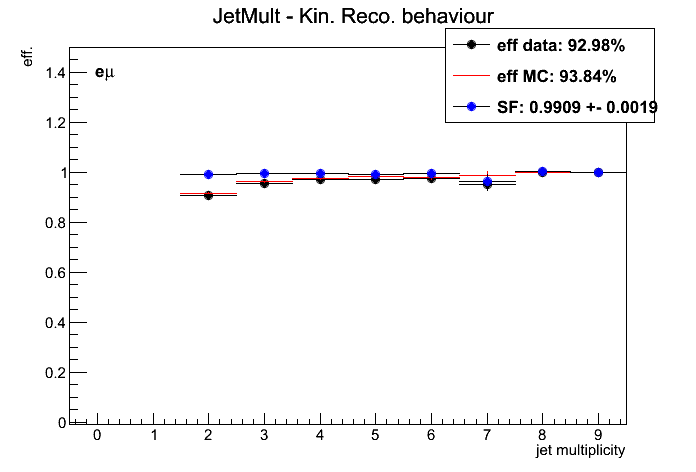
\includegraphics[width=0.49\textwidth]{05_kinReco/plots/eff_SF/KinRecoEff_JetMult.png}
\end{subfigure}
\begin{subfigure}
  \centering
  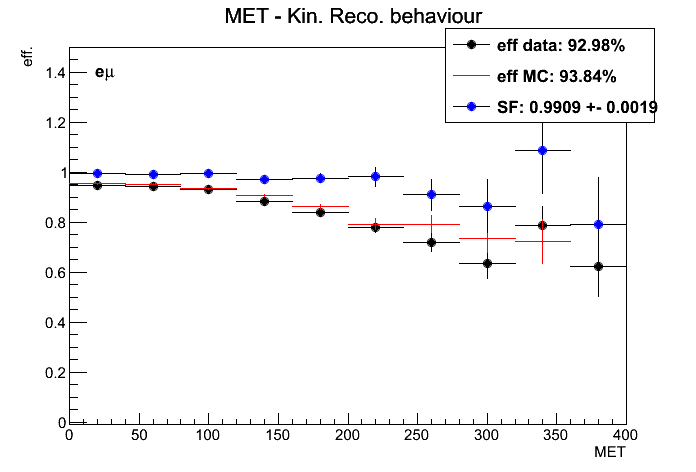
\includegraphics[width=0.49\textwidth]{05_kinReco/plots/eff_SF/KinRecoEff_MET.png}
\end{subfigure}
\begin{subfigure}
  \centering
  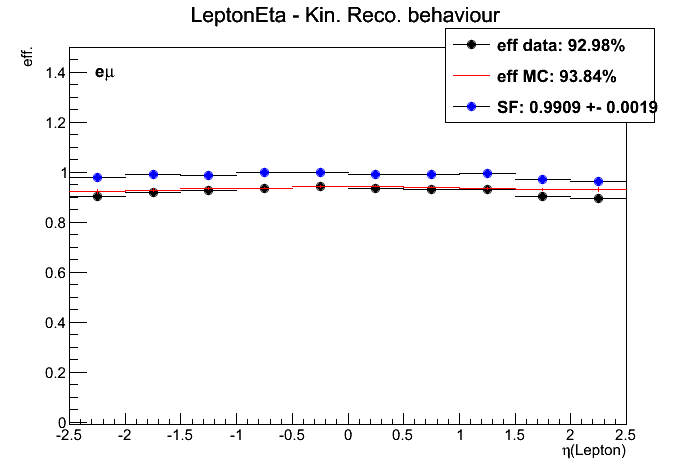
\includegraphics[width=0.49\textwidth]{05_kinReco/plots/eff_SF/KinRecoEff_LeptonEta.png}
\end{subfigure}
\begin{subfigure}
  \centering
  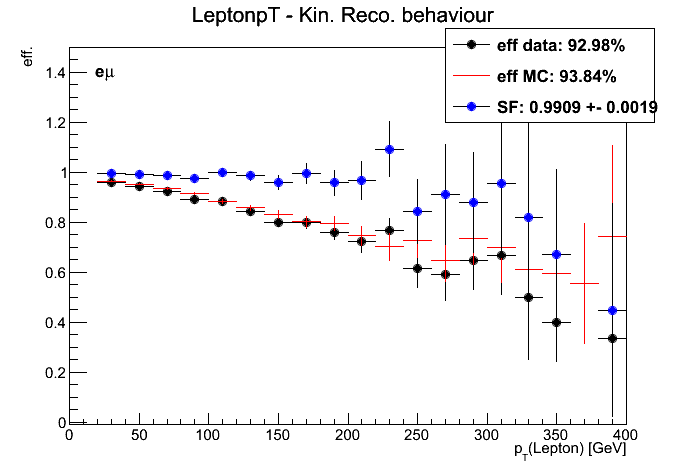
\includegraphics[width=0.49\textwidth]{05_kinReco/plots/eff_SF/KinRecoEff_LeptonpT.png}
\end{subfigure}
\begin{subfigure}
  \centering
  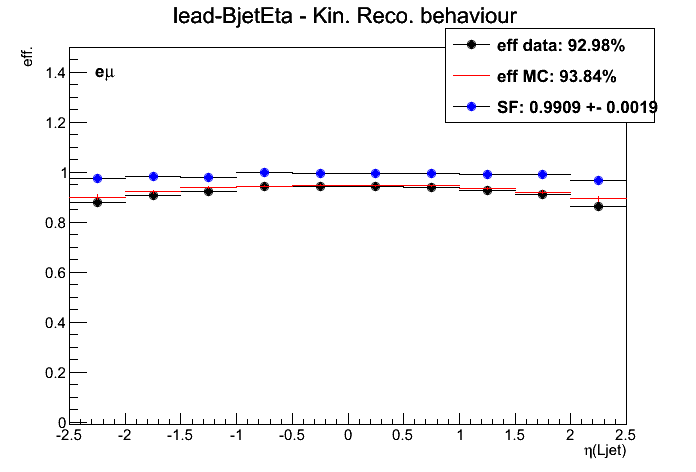
\includegraphics[width=0.49\textwidth]{05_kinReco/plots/eff_SF/KinRecoEff_JetEta.png}
\end{subfigure}
\begin{subfigure}
  \centering
  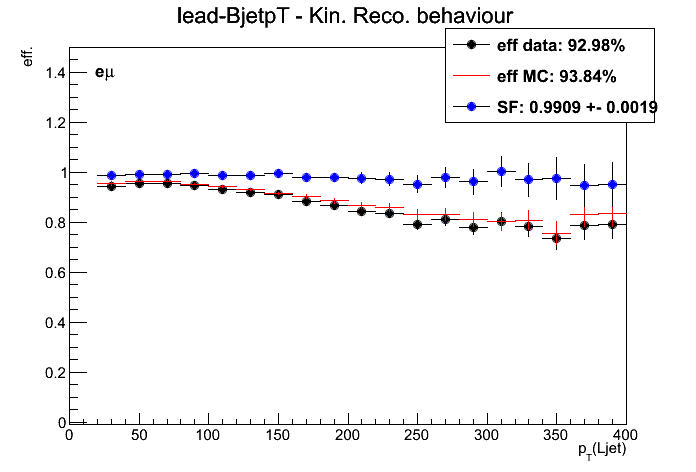
\includegraphics[width=0.49\textwidth]{05_kinReco/plots/eff_SF/KinRecoEff_JetpT.png}
\end{subfigure}
\caption{The efficiencies and scale factors for the $t\bar{t}$ kinematics reconstruction procedure in bins of the jet multiplicity in the event (top left),
         missing transverse energy (top right), lepton pseudorapidity (middle left) and transverse momentum (middle right) and $b$-jet pseudorapidity (bottom left) 
         and transverse momentum (bottom right). The efficiencies in the data 
         are marked with black dots, efficiencies in MC simulations are red lined and the scale factors (ratio of data and MC efficiencies) are plotted with the blue dots.
         The simulated MC samples contain $t\bar{t}$ signal and the backgrounds.}
\label{fig:EffSF}
\end{figure}

The scatter plots in Fig. \ref{fig:ScatterPl} show the correlation between the kinematic variables of the $t$ or $t\bar{t}$ system on the reconstructed and generated
levels of the $t\bar{t}$ signal MC.
% after the selection and kinematic reconstruction in the simulated
% signal and the actual characteristics of the $t\bar{t}$ system and decay on the particle level. 
There are no shifts and trends observed, thus showing 
the trustful behavior of the kinematic reconstruction algorithm.

\begin{figure}[t]
\centering
\begin{subfigure}
  \centering
  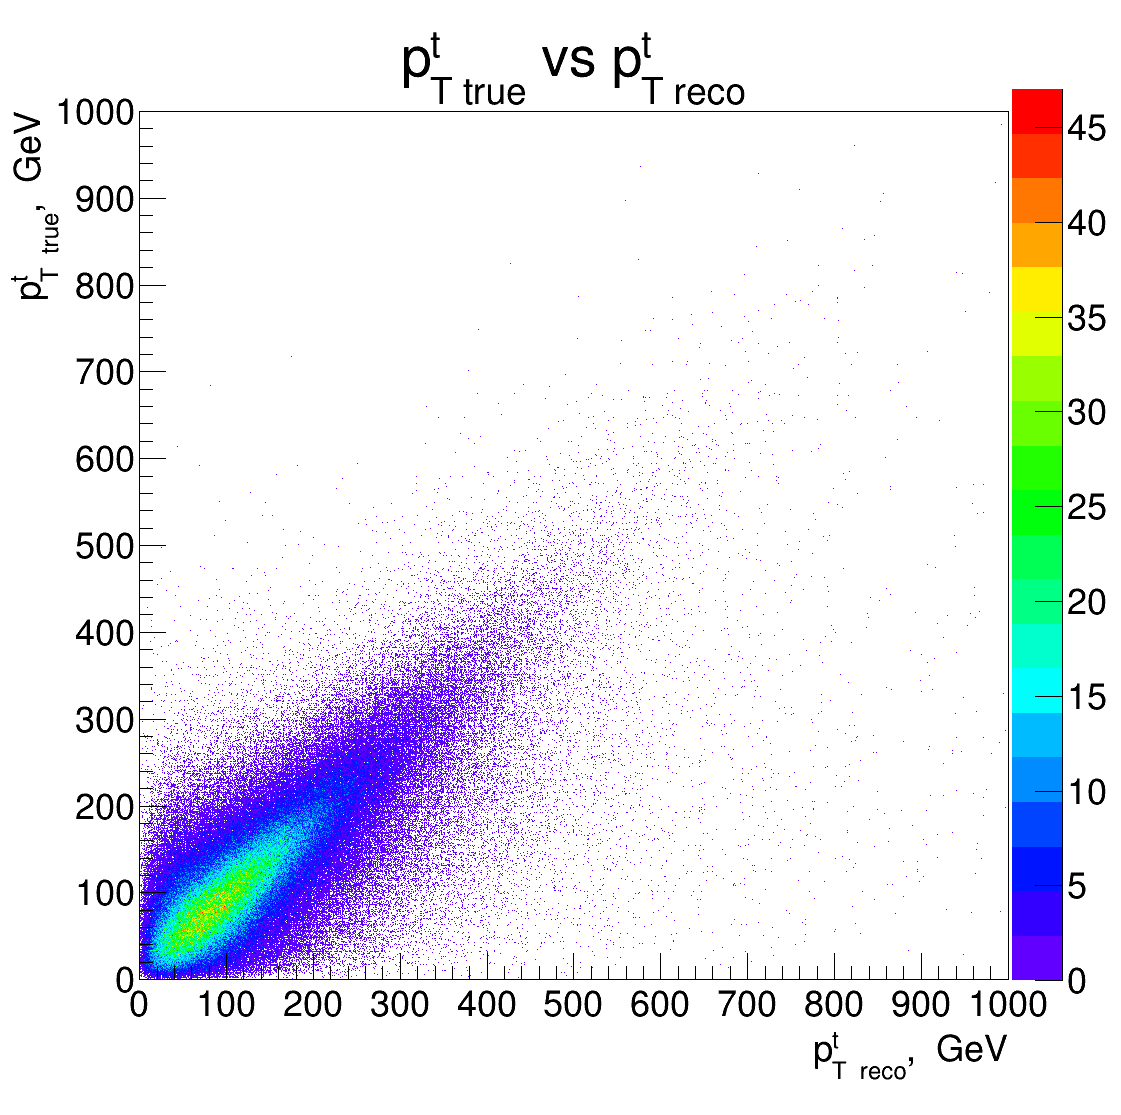
\includegraphics[width=0.45\textwidth]{05_kinReco/plots/scatter/pt-t.png}
\end{subfigure}
\begin{subfigure}
  \centering
  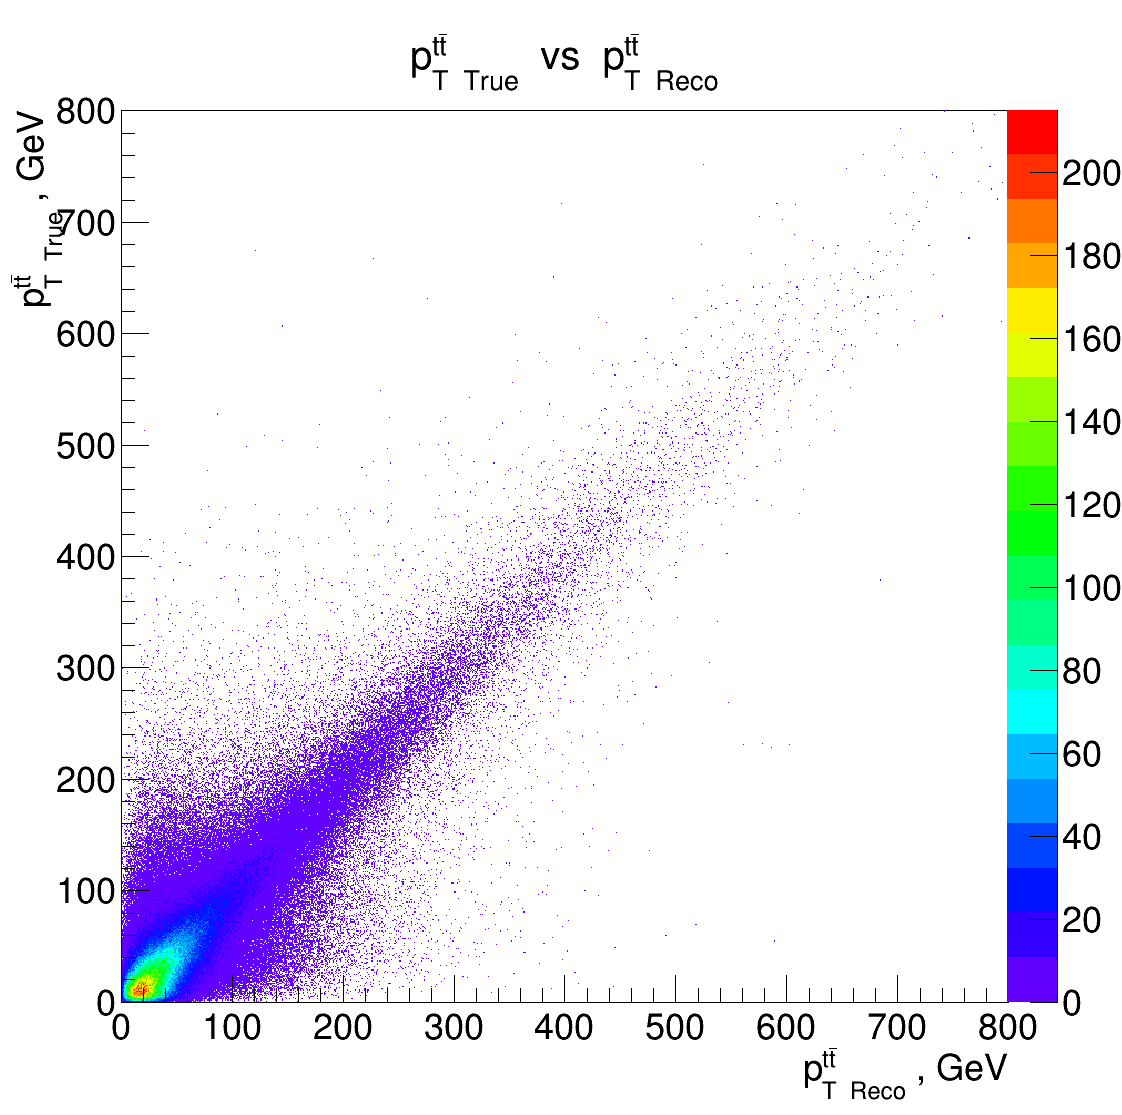
\includegraphics[width=0.45\textwidth]{05_kinReco/plots/scatter/pTtt-scaterPlot.png}
\end{subfigure}
\begin{subfigure}
  \centering
  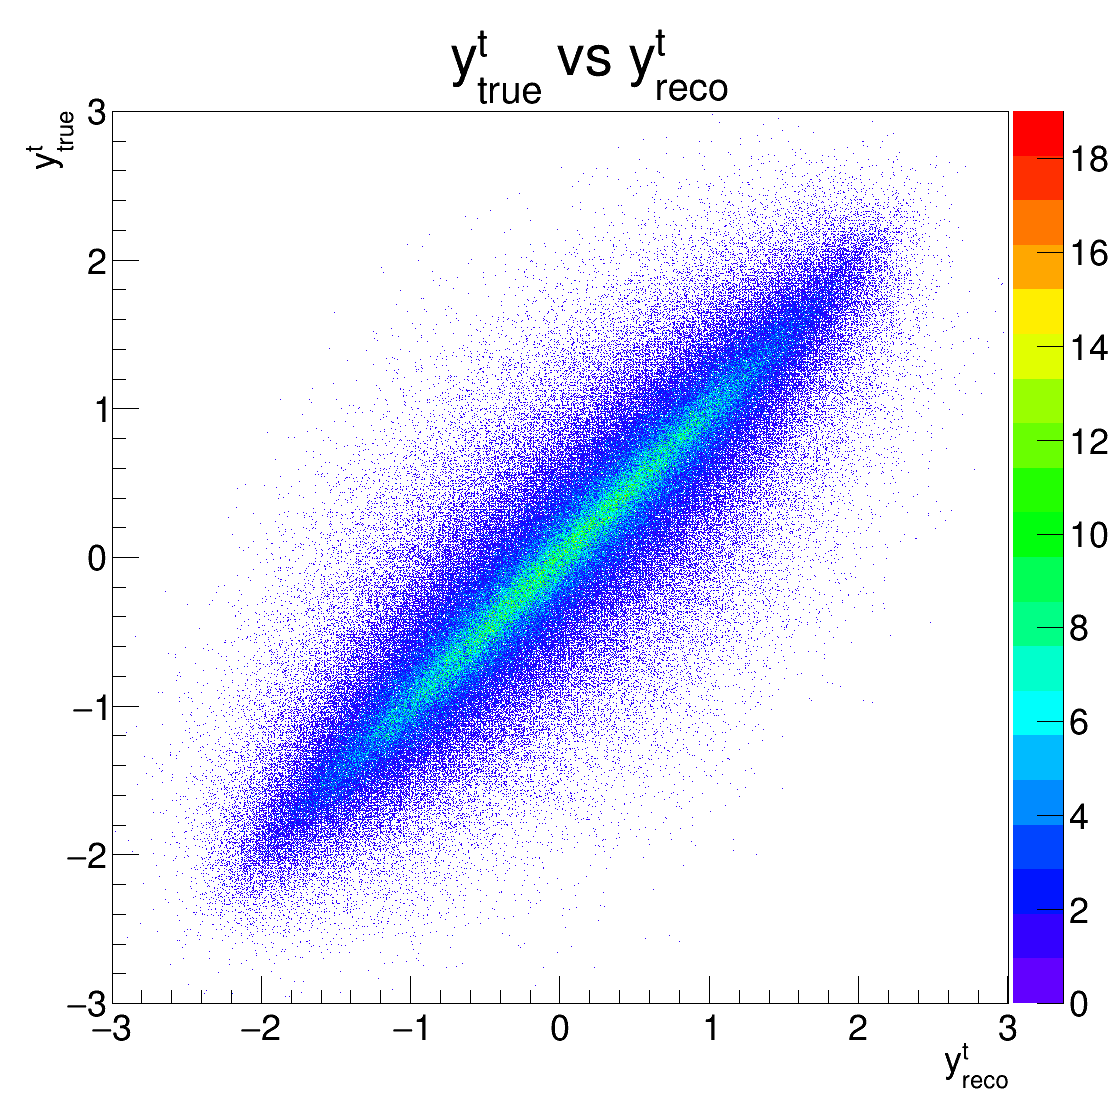
\includegraphics[width=0.45\textwidth]{05_kinReco/plots/scatter/y-t.png}
\end{subfigure}
\begin{subfigure}
  \centering
  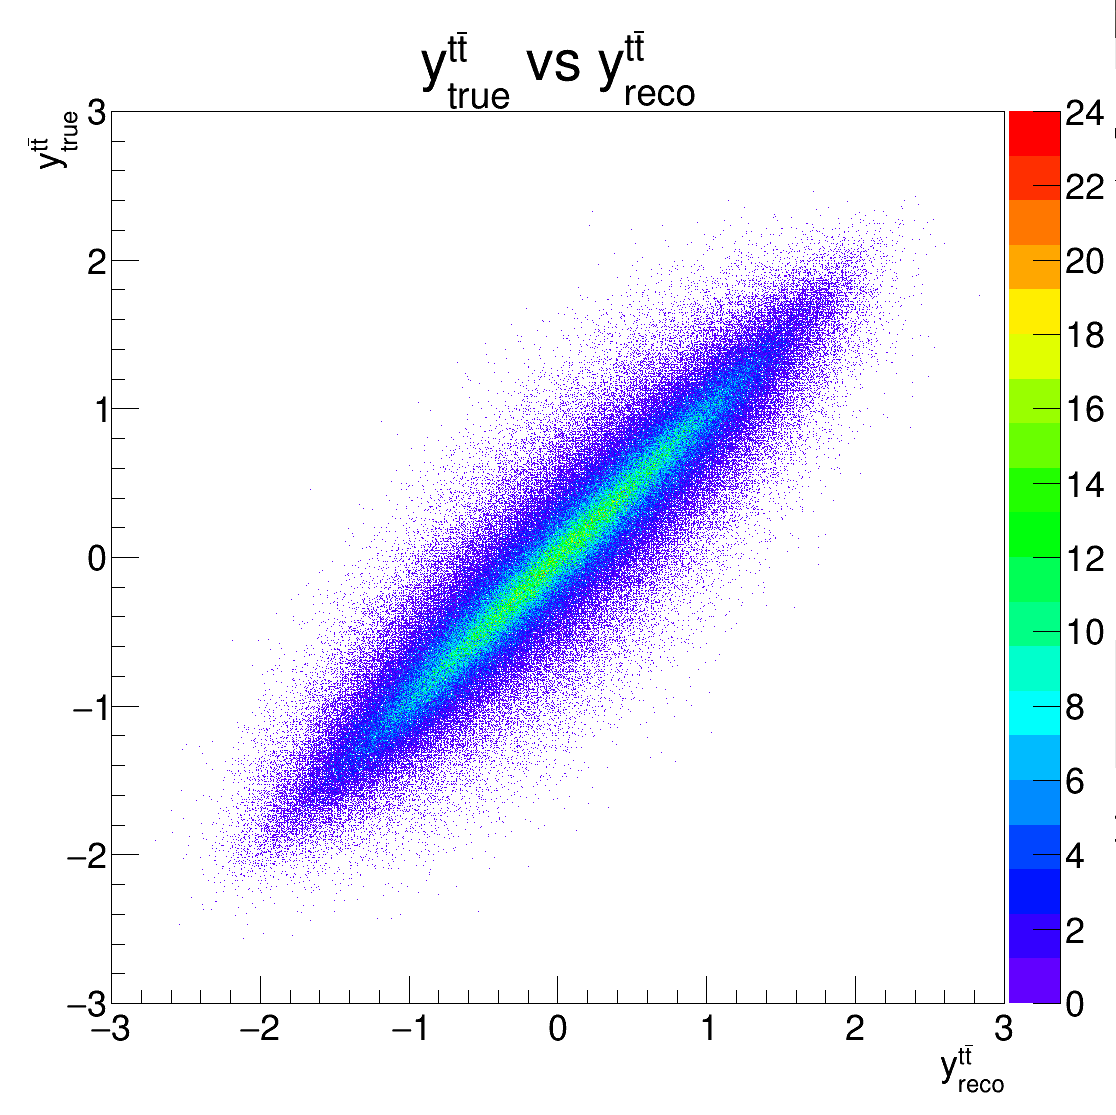
\includegraphics[width=0.45\textwidth]{05_kinReco/plots/scatter/y-tt.png}
\end{subfigure}
\begin{subfigure}
  \centering
  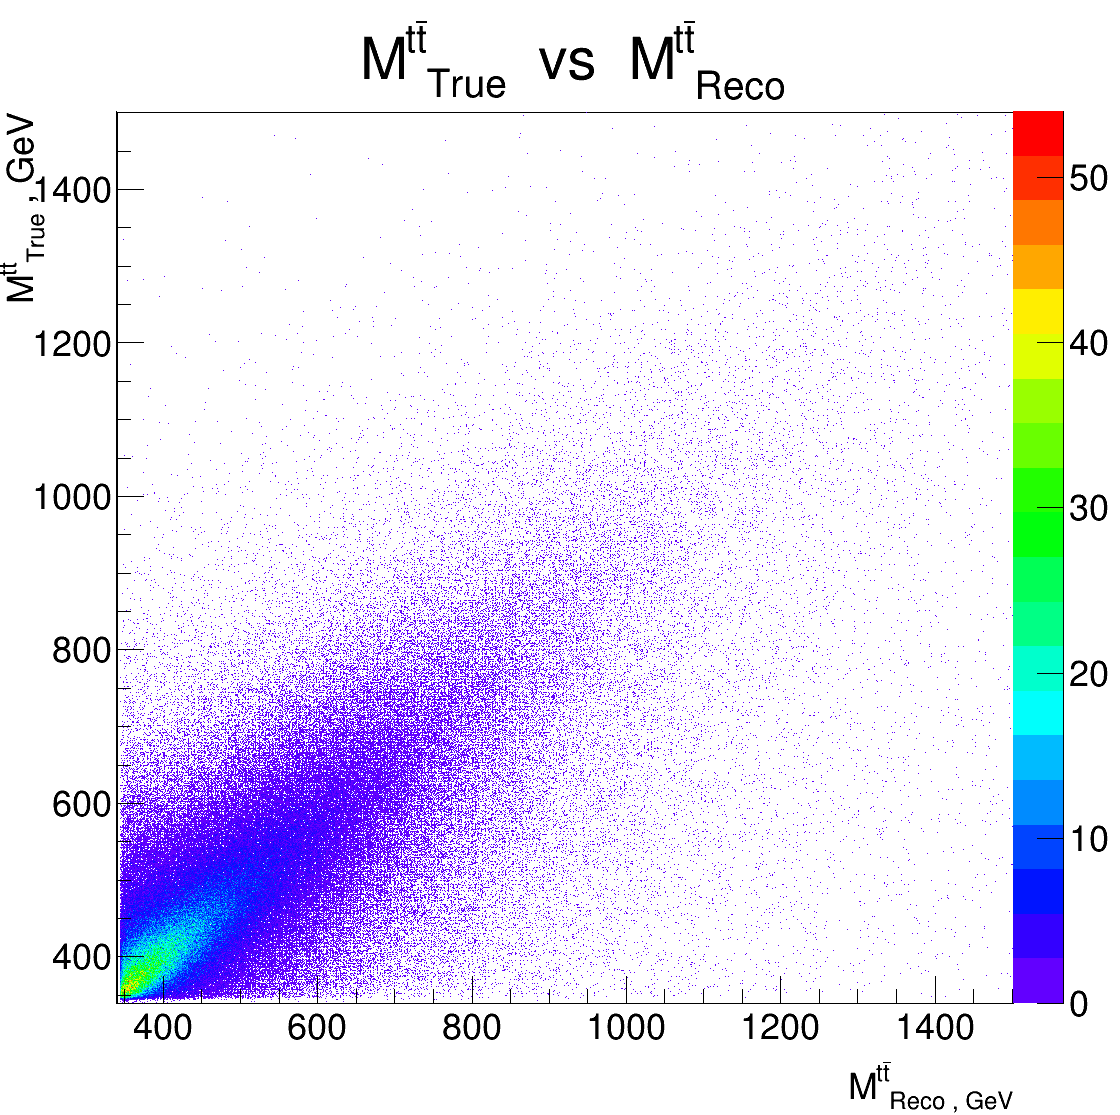
\includegraphics[width=0.45\textwidth]{05_kinReco/plots/scatter/mtt-scaterPlot.png}
\end{subfigure}
\caption{Plots which show the reconstructed vs. generated variables: the transverse momentum of the $t$ and $t\bar{t}$ (top left and right respectively), 
        the rapidity of the $t$ and $t\bar{t}$ (middle left and right respectively) and the invariant mass of the $t\bar{t}$ system, obtained from the 
        signal MC.}
\label{fig:ScatterPl}
\end{figure}

This kinematic reconstruction method is an alternative to the kinematic reconstruction utilized in the measurement of the single differential $t\bar{t}$
production cross sections in the dilepton channel at $\sqrt{s} = $7 TeV \cite{Chatrchyan:2012saa}, where no smearing of the leptons and 
jets energies and directions were performed, and on the other hand the top-quark mass was scanned. The kinematic reconstruction method described
in this chapter has a 50\% lower inefficiency compared to the previous method.

\section{Control Distributions}

The kinematic reconstruction method shows good results over the complete kinematic range of the top system. The Fig. \ref{fig:CPkinTop} shows
the control distributions of the kinematic quantities of the top quark system. The distribution of the transverse momentum of the top quark
shows a good agreement between experimental data and simulation at small and intermediate $p_{T}$. However the higher $p_{T}$ range is not well
described by the MC. The measured spectrum in $p_{T}$ is overall softer than the simulation. The rapidity is well described by the simulation in the central region, 
whereas for the edges MC slightly underestimates the data -- the simulation is more central.
An overall good agreement is observed in the  $x_{1}$\footnote{ $x_{1}$ is a fraction of a proton momentum transfered to a $t$ quark} 
distribution.

\begin{figure}[h]
\centering
\begin{subfigure}
  \centering
  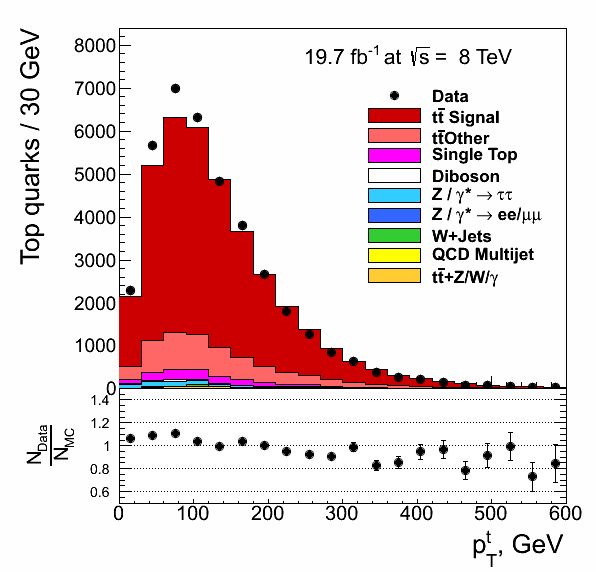
\includegraphics[width=0.49\textwidth]{/home/dolinska/Dropbox/desy_plots/Thesis/Jenya/05_kinReco/plots/CP-Plots/newCP/CP_top_pt.pdf}
\end{subfigure}
\begin{subfigure}
  \centering
  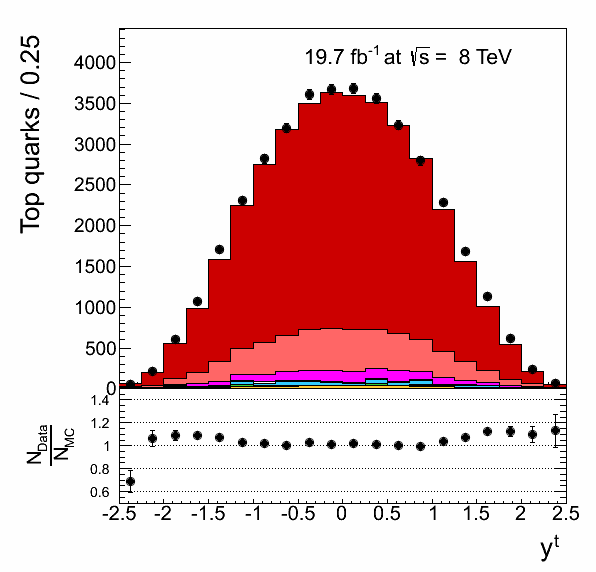
\includegraphics[width=0.49\textwidth]{/home/dolinska/Dropbox/desy_plots/Thesis/Jenya/05_kinReco/plots/CP-Plots/newCP/CP_top_rapidity.pdf}
\end{subfigure}
\begin{subfigure}
  \centering
  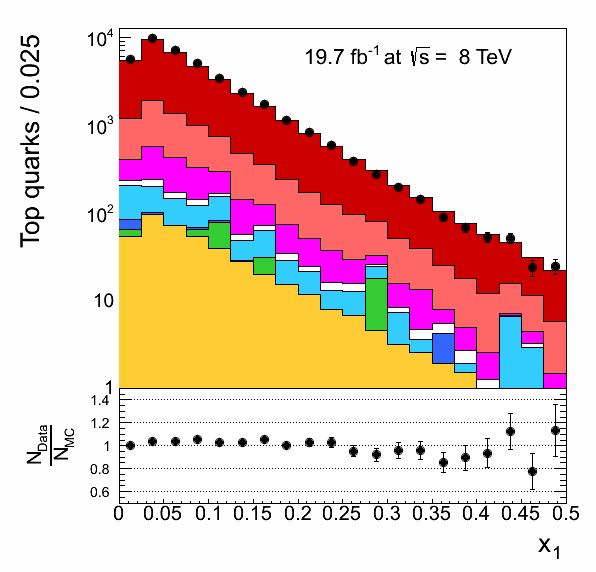
\includegraphics[width=0.49\textwidth]{/home/dolinska/Dropbox/desy_plots/Thesis/Jenya/05_kinReco/plots/CP-Plots/newCP/CP_x1.pdf}
\end{subfigure}
\caption{Control distributions of the top quark $p_{T}$ (top left), rapidity (top right) and  $x_{1}$ in the events 
 after the kinematic reconstruction. The experimental data with the error bars corresponding to the statistical uncertainties
 and simulated distributions of signal and different background are plotted. Each of the plots show in the bottom panel the MC-to-data yield ratio distributions. 
 The distributions are presented for the $t$ quark only.}
\label{fig:CPkinTop}
\end{figure}

In figure \ref{fig:CPkinTTbar} the control distributions of the kinematic variables of the $t\bar{t}$ system are presented. The transverse momentum is overall
well described by the simulation. A slight data excess is observed in central rapidity $y^{t\bar{t}}$ and the edges have also slightly worse agreement between
experimental data and MC. The invariant mass of the $t\bar{t}$ system is reasonably well described by the simulation for the complete mass range -- in the region 
of 800-1000 GeV the simulation is a bit lower than data.

\begin{figure}[h]
\centering
\begin{subfigure}
  \centering
  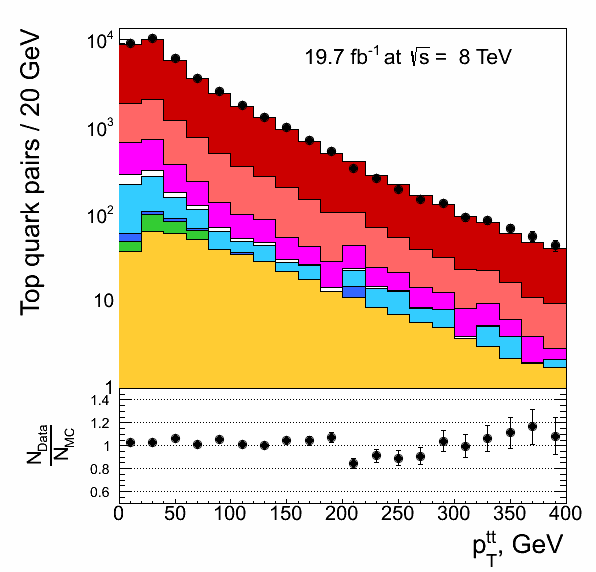
\includegraphics[width=0.49\textwidth]{/home/dolinska/Dropbox/desy_plots/Thesis/Jenya/05_kinReco/plots/CP-Plots/newCP/CP_ttbar_pt.pdf}
\end{subfigure}
\begin{subfigure}
  \centering
  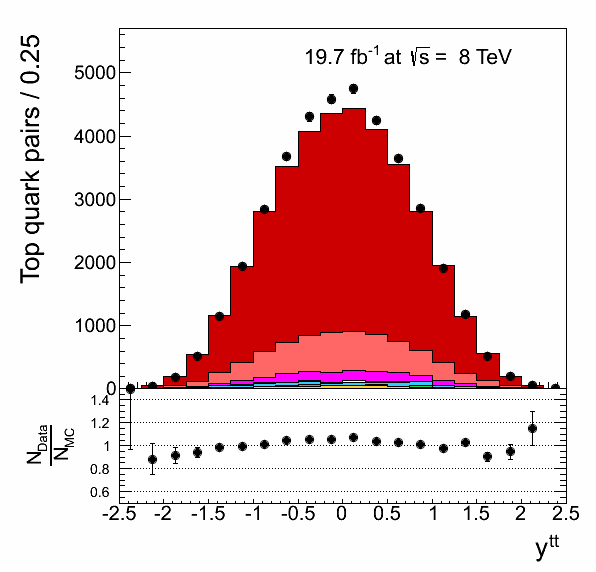
\includegraphics[width=0.49\textwidth]{/home/dolinska/Dropbox/desy_plots/Thesis/Jenya/05_kinReco/plots/CP-Plots/newCP/CP_ttbar_rapidity.pdf}
\end{subfigure}
\begin{subfigure}
  \centering
  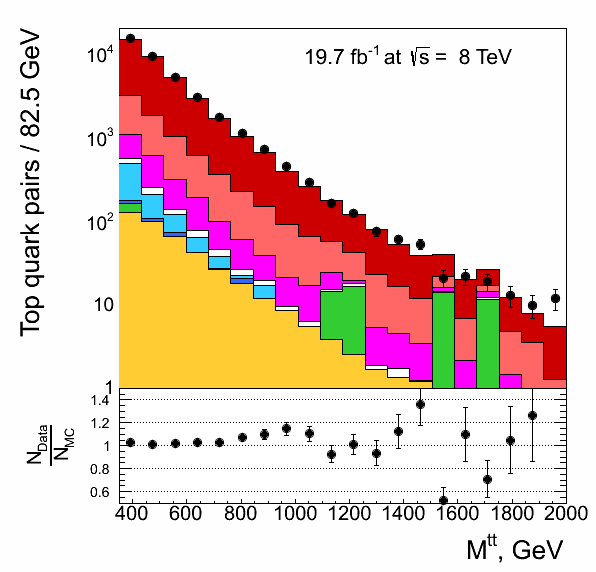
\includegraphics[width=0.49\textwidth]{/home/dolinska/Dropbox/desy_plots/Thesis/Jenya/05_kinReco/plots/CP-Plots/newCP/CP_ttbar_mass.pdf}
\end{subfigure}
\caption{Control distributions of the $p_{T}$ (top left), rapidity (top right) and invariant mass of the $t\bar{t}$ system in the events 
 after the kinematic reconstruction. Other details as in Fig. \ref{fig:CPkinTop}.}
\label{fig:CPkinTTbar}
\end{figure}

\section{Usage of the Kinematic Reconstruction}

Apart of this work, the kinematic reconstruction as described in this chapter has also been implemented into the analysis, which measured the single differential $t\bar{t}$
production cross sections in the dilepton channel at $\sqrt{s} = $8 TeV, TOP-12-028 \cite{Khachatryan:2015oqa} \cite{TWikiTOP12028}. 

The results obtained in TOP-12-028 \cite{Khachatryan:2015oqa} \cite{TWikiTOP12028} exploiting the kinematic reconstruction are presented 
in Fig. \ref{fig:xsec_top12028}.

\begin{figure}[h]
\centering
\begin{subfigure}
  \centering
  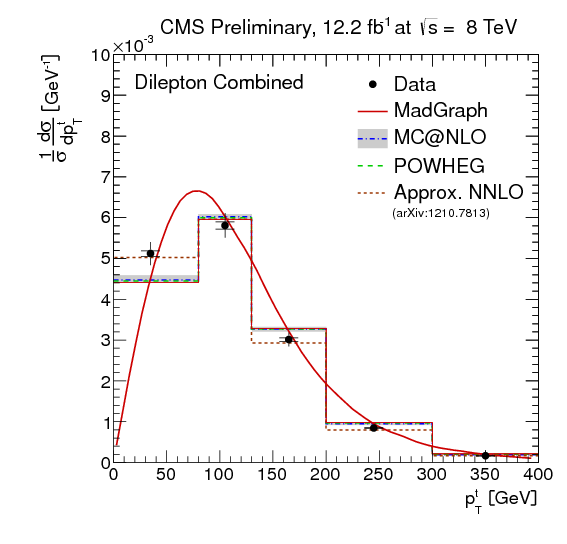
\includegraphics[width=0.49\textwidth]{05_kinReco/plots/DiffXS_HypToppT.png}
\end{subfigure}
\begin{subfigure}
  \centering
  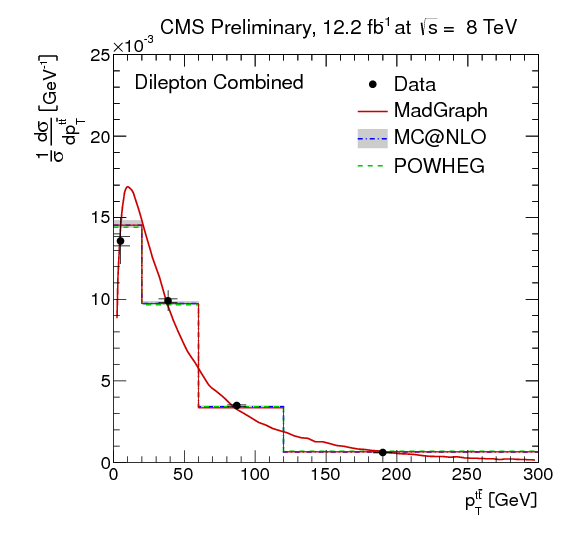
\includegraphics[width=0.49\textwidth]{05_kinReco/plots/DiffXS_HypTTBarpT.png}
\end{subfigure}
\caption{Normalised differential $t\bar{t}$ production cross section as a function of the $p_{T}$ of the top quarks or antiquarks and $t\bar{t}$-pairs. 
         The superscript 't' refers to both top quarks and antiquarks. The inner (outer) error bars indicate the statistical (combined statistical and 
         systematic) uncertainty. The measurement is compared to predictions from \MG, \Powheg and \MCNLO Monte Carlo generators. The \MG prediction is 
         shown both as a curve and as a binned histogram. The figures are taken from \cite{TWikiTOP12028} \cite{Khachatryan:2015oqa}.}
\label{fig:xsec_top12028}
\end{figure}